\section{Results}
\label{sec:results}

All numbers are differences in fitness (Section~\ref{sec:evolution}), averaged over evaluation worlds within each training seed; intervals are percentile bootstrap intervals over training seeds (Section~\ref{sec:protocol}). Figure~\ref{fig:forest} summarises the main confirmatory comparisons and Table~\ref{tab:confirmatory} lists every hypothesis with its formal outcome; Appendix Table~\ref{tab:tiers} gives the tiered reading. We describe the results in the order of the questions they answer; a result is called \emph{conditional} when it holds only under a stated delay, dialect or cue structure.

\begin{figure}[t]
\centering
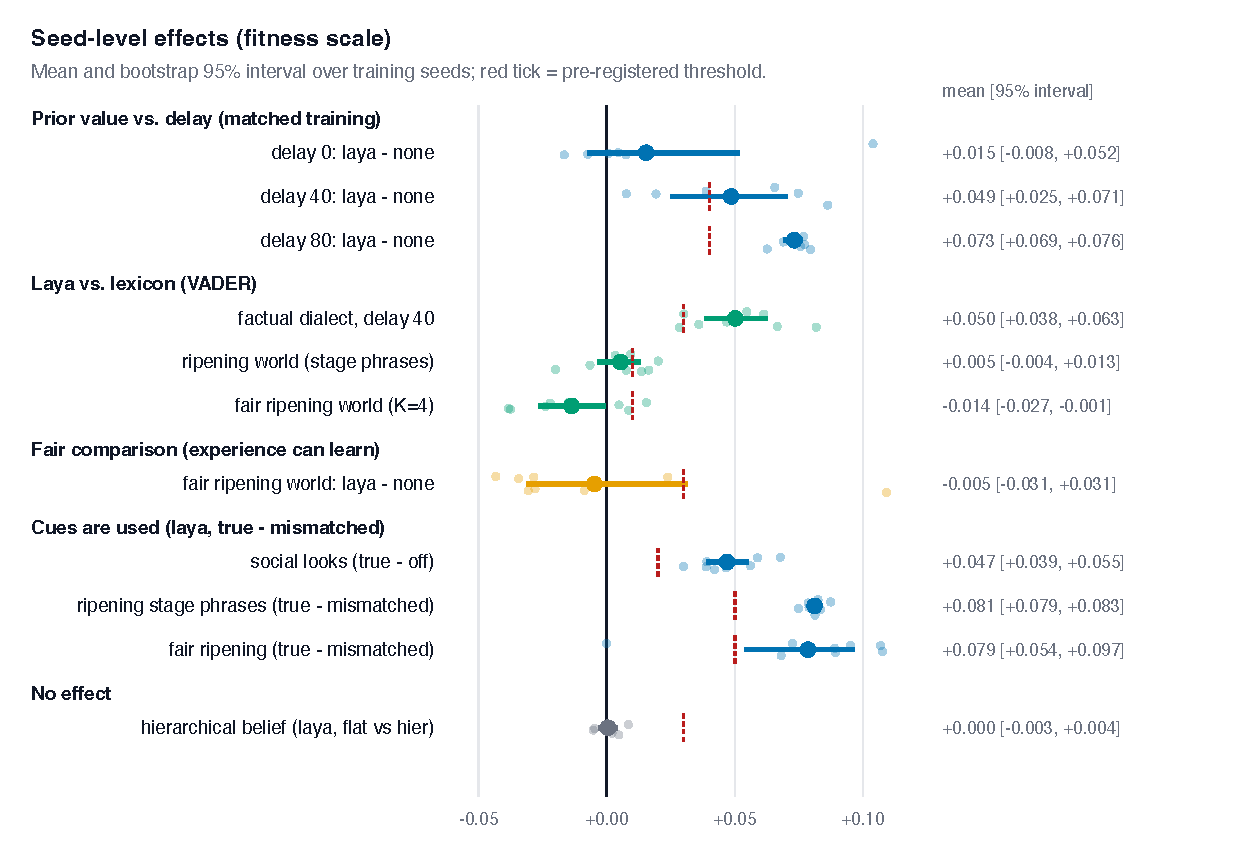
\includegraphics[width=\textwidth]{figures/fig1_forest.pdf}
\caption{Seed-level effects of the main confirmatory comparisons (fitness scale). Large dots are means with bootstrap 95\% intervals over training seeds, small dots are individual seeds and red ticks are the pre-registered thresholds. Rows from the same group answer the same question; the grey row is a null result.}
\label{fig:forest}
\end{figure}

\begin{table}[t]\centering\small\caption{Confirmatory comparisons (pre-registrations 04--11). Mean and 95\% percentile bootstrap interval over training seeds; $p$ is the exact one-sided sign-flip test (non-inferiority rows are tested against the margin). Threshold is the pre-registered effect size.}\label{tab:confirmatory}
\begin{tabular}{@{}llrrrrll@{}}\toprule
Pre-reg. & Comparison & $n$ & Mean & 95\% interval & $p$ & Threshold & Formal outcome \\\midrule
04 & Delay 40: laya $-$ none (mismatched training) & 8 & +0.032 & [+0.025, +0.042] & 0.0039 & +0.04 & not supported (magnitude) \\
04 & Prior value grows with delay (D40 $-$ D0) & 8 & +0.143 & [+0.120, +0.168] & 0.0039 & +0.03 & not claimed (tied $p$) \\
06 & Delay 0: laya $-$ none (non-inferiority) & 6 & +0.015 & [-0.008, +0.052] & 0.0156 & -0.04 & supported \\
06 & Delay 40: laya $-$ none (matched training) & 6 & +0.049 & [+0.025, +0.071] & 0.0156 & +0.04 & supported \\
06 & Hierarchical belief, laya (deception 0.40) & 6 & +0.000 & [-0.003, +0.004] & 0.4375 & +0.03 & not supported \\
07 & Factual dialect, delay 40: laya $-$ vader & 8 & +0.050 & [+0.038, +0.063] & 0.0039 & +0.03 & supported \\
07 & Held-out dialect, delay 80: laya $-$ none & 8 & +0.073 & [+0.069, +0.076] & 0.0039 & +0.04 & supported \\
07 & Prior value grows with delay (d80 $-$ d40) & 8 & +0.035 & [+0.025, +0.046] & 0.0039 & +0.02 & supported \\
08 & Gap widening: (laya $-$ vader) factual vs.\ sentiment training & 8 & -0.002 & [-0.008, +0.006] & 0.6328 & +0.02 & not supported \\
08 & Factual training: laya $-$ none (factual dialect) & 8 & +0.032 & [+0.026, +0.038] & 0.0039 & +0.05 & not supported (magnitude) \\
08 & Transfer: factual-trained, held-out dialect, laya $-$ vader (non-inferiority) & 8 & +0.062 & [+0.058, +0.066] & 0.0039 & -0.02 & supported \\
09 & Social looks: true $-$ absent (laya) & 8 & +0.047 & [+0.039, +0.055] & 0.0039 & +0.02 & supported \\
09 & Social looks: absent $-$ mismatched (laya) & 8 & +0.101 & [+0.091, +0.111] & 0.0039 & +0.05 & supported \\
09 & Social gain: laya $-$ vader & 8 & +0.025 & [+0.007, +0.044] & 0.0273 & +0.01 & supported \\
10 & Ripening: laya $-$ none (true cues) & 8 & +0.060 & [+0.044, +0.082] & 0.0039 & +0.03 & supported \\
10 & Ripening: true $-$ mismatched (laya) & 8 & +0.081 & [+0.079, +0.083] & 0.0039 & +0.05 & supported \\
10 & Ripening: laya $-$ vader & 8 & +0.005 & [-0.003, +0.013] & 0.1328 & +0.01 & not supported \\
11 & Fair ripening ($K{=}4$): laya $-$ none & 8 & -0.005 & [-0.031, +0.032] & 0.5938 & +0.03 & not supported \\
11 & Fair ripening: true $-$ mismatched (laya) & 8 & +0.079 & [+0.053, +0.097] & 0.0039 & +0.05 & supported \\
11 & Fair ripening: laya $-$ vader & 8 & -0.014 & [-0.027, -0.000] & 0.9492 & +0.01 & not supported \\
\bottomrule\end{tabular}\end{table}


\subsection{The frozen model reads meaning, a lexicon reads sentiment}
\label{sec:res-quality}
Before any individual is evaluated, we measured how well each prior source separates nutritive from toxic descriptions (area under the ROC curve; 0.5 is chance; Figure~\ref{fig:auc}). On the first 1,500 descriptions of the held-out field-notes dialect, \laya{} reaches 0.909, the VADER lexicon 0.689, an author-written generic lexicon 0.720 and a lexicon trained on the training dialect 0.778; the shuffled control is at chance (0.498). On the factual dialect (4,000 descriptions), whose clues are neutral in tone, \laya{} keeps 0.775 while the lexicons fall to 0.583 (VADER) and 0.535 (generic); the difference \laya{}$-$VADER is $+0.192$ (95\% interval $[0.170,0.212]$; pre-registration 05, supported). The lexicons' high accuracy on toxic descriptions in this dialect is an artefact of answering ``avoid'' almost always: they are correct on only 11--38\% of nutritive descriptions. This is a statement about the \emph{quality of the prior}; whether it translates into better individuals is the subject of the following sections.

\begin{figure}[t]
\centering
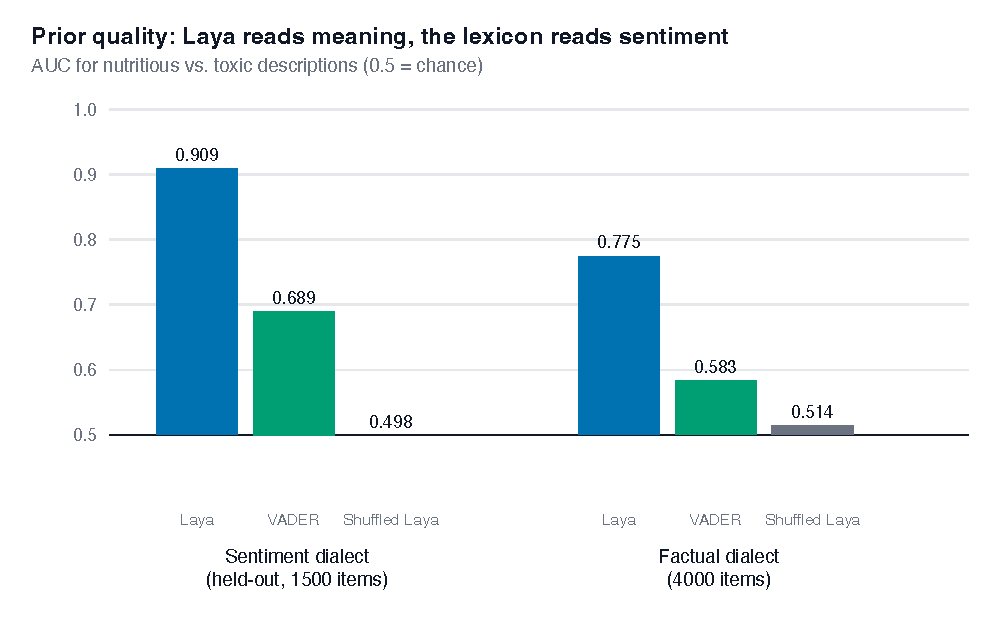
\includegraphics[width=0.75\textwidth]{figures/fig4_auc.pdf}
\caption{Quality of the prior: AUC for nutritious versus toxic descriptions (held-out field-notes dialect, 1,500 items; factual dialect, 4,000 items).}
\label{fig:auc}
\end{figure}

\subsection{The value of the prior depends on the delay of consequences}
\label{sec:res-delay}
\paragraph{An artefact of mismatched training.}
In pre-registration 04 the individuals were trained in worlds with a delay of 20 ticks and a deception rate of at most 0.25, and evaluated at delays 0 and 40 and at deception rates 0.25 and 0.40 (eight seeds). Without delay, individuals with the \laya{} prior were \emph{worse} than individuals with no prior in all eight seeds ($-0.085$ at deception 0.25, $-0.136$ at 0.40), while at delay 40 and deception 0.25 they were better ($+0.096$, 8/8). Read alone, this suggests that a prior harms when feedback is immediate.

\paragraph{Matched training removes the harm.}
In pre-registration 06 every training and evaluation world of a condition shares the same delay (48 runs, six seeds). Without delay the difference is $+0.015$ (interval $[-0.008,+0.052]$; four of six seeds positive); non-inferiority to a margin of $-0.04$ is supported, but the effect is not positive in every seed, so the correct reading is ``not harmful'', not ``helpful''. At delay 40 the difference is $+0.049$ ($[+0.025,+0.071]$, six of six seeds positive; supported). The harm in pre-registration 04 therefore came from evaluating individuals in worlds that differ from the ones they evolved in.

\paragraph{The value grows with the delay.}
In pre-registration 07 (eight new seeds, matched training, held-out dialect) the difference is $+0.038$ ($[+0.028,+0.048]$) at delay 40 and $+0.073$ ($[+0.069,+0.077]$) at delay 80; the per-seed values at delay 80 lie between 0.062 and 0.080. The growth with delay, (delay 80)$-$(delay 40), is $+0.035$ ($[+0.025,+0.046]$, 8/8; supported). At delay 80 individuals with the prior bit toxic food 386 times on average against 753 without it. Figure~\ref{fig:delay} shows the trend across the two pre-registrations. \textbf{This trend has to be read together with the behaviour of the no-prior genomes at delay 80.} On a shared sample of 12 held-out worlds, six of the eight no-prior genomes scored exactly as the blind rule that eats everything it reaches (fitness 0.253, 664 toxic bites, survival 0.357); the other two scored 0.264 and 0.266. At delay 40 all eight scored above the blind rule (0.288 to 0.305). In most seeds at delay 80, therefore, the experience-only learner did not learn to avoid anything, and part of the growth of the prior's value with the delay is the failure of this learner at long delays, not only the benefit of the prior. The blind rule and the oracle scored 0.253 and 0.563 on the same worlds, so individuals with the prior (0.352 to 0.377 across seeds) closed about a third of the gap between them. On the factual pool the corresponding differences are smaller ($+0.016$, interval containing zero, at delay 40; $+0.037$ at delay 80; descriptive). The pre-registration-04 hypothesis that the benefit at delay 40 reaches $+0.04$ was not supported: the mean was $+0.032$ in 8/8 seeds, and the interval $[+0.025,+0.042]$ contains the threshold (direction confirmed, magnitude unclear).

\begin{figure}[t]
\centering
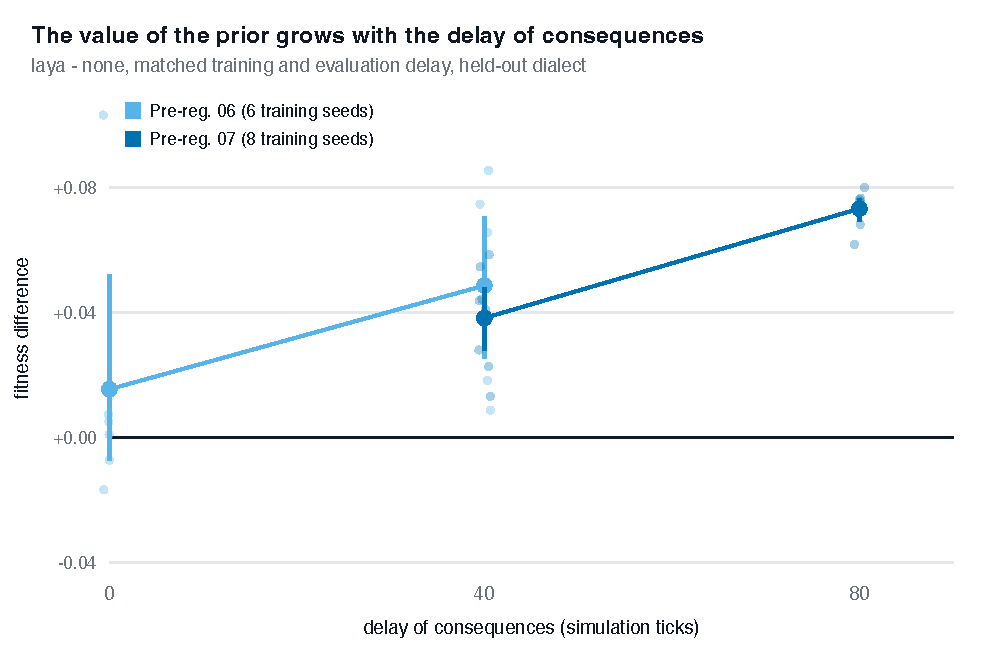
\includegraphics[width=0.75\textwidth]{figures/fig2_delay.pdf}
\caption{Fitness difference (\texttt{laya}$-$\texttt{none}) as a function of the consequence delay under matched training and evaluation, held-out dialect. Large dots are means with bootstrap intervals; small dots are training seeds.}
\label{fig:delay}
\end{figure}

\subsection{\laya{} versus a lexicon: only where meaning is needed}
\label{sec:res-lexicon}
In pre-registration 07, on the factual dialect at delay 40, individuals with the \laya{} prior beat individuals with the VADER prior by $+0.050$ ($[+0.038,+0.063]$, 8/8; supported). In the same worlds the VADER prior was worse than no prior ($-0.034$, seven of eight seeds negative; descriptive). On the held-out field-notes dialect, where the lexicon can read the text, the differences are smaller ($+0.025$ at delay 40, $+0.027$ at delay 80; descriptive, not tested).

Pre-registration 08 asked whether training on the factual dialect would widen the gap, and whether what is learned transfers. The gap did not widen: the difference \laya{}$-$VADER on the factual pool was $+0.029$ after sentiment-dialect training and $+0.028$ after factual-dialect training (change $-0.0015$, $[-0.008,+0.006]$; not supported). The advantage of the prior over no prior after factual training was $+0.032$ in 8/8 seeds, below the pre-registered threshold of 0.05 (not supported on magnitude). What \emph{did} differ was transfer to the held-out dialect: \laya{} individuals trained on the factual dialect scored 0.333 there, the same as those trained on the sentiment dialect (0.334), while VADER individuals fell from 0.307 to 0.271, so that \laya{}$-$VADER on the held-out pool grew from $+0.027$ to $+0.062$ ($[+0.058,+0.066]$, 8/8; the pre-registered non-inferiority test was supported). A plausible reading, which we have not tested, is that the reliability of a lexicon varies from dialect to dialect, so the trust that evolution assigns to it in one dialect does not carry over, whereas the reliability of the frozen model is stable and so is the trust learned for it.

In the ripening worlds (Section~\ref{sec:res-cues}), where the stage phrases carry sentiment that a lexicon can read, the two priors were indistinguishable ($+0.005$, $[-0.004,+0.013]$; not supported) or slightly in favour of the lexicon ($-0.014$ in the fair world, $[-0.027,-0.0005]$).

\subsection{Language cues are used, and wrong cues cost}
\label{sec:res-cues}
We evaluated the same individuals under three cue conditions (true, absent, mismatched; Section~\ref{sec:ecology}) with phrases that were never seen in training (Figure~\ref{fig:cues}).

\begin{figure}[t]
\centering
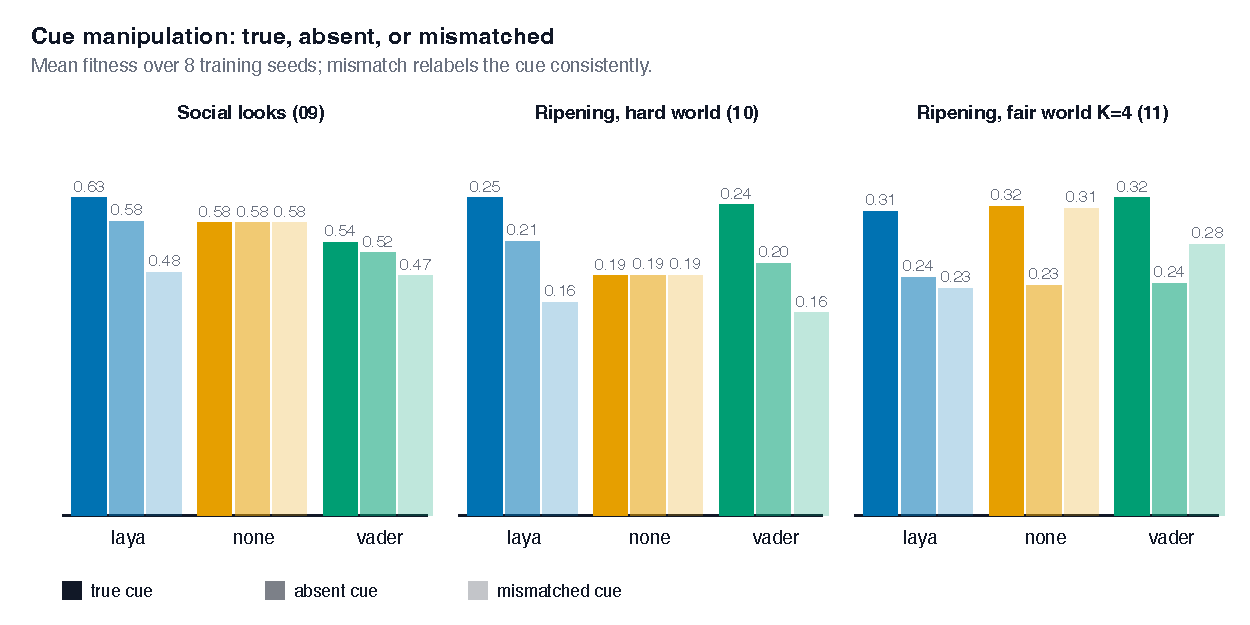
\includegraphics[width=\textwidth]{figures/fig3_cues.pdf}
\caption{Mean fitness under true, absent and mismatched cues, for individuals with each prior source (eight seeds). A mismatch relabels the cue consistently, so individuals that only learn from experience are unaffected; individuals that read the cue lose.}
\label{fig:cues}
\end{figure}

\paragraph{Social appearance (pre-registration 09).}
Individuals with the \laya{} prior scored 0.629 with true appearances, 0.582 with none and 0.481 with mismatched ones. The gain of true over absent appearances is $+0.047$ ($[+0.039,+0.055]$, 8/8; supported) and the cost of mismatched versus absent appearances $+0.101$ ($[+0.091,+0.111]$, 8/8; supported). Individuals with no prior were identical in all three conditions (0.579), as they cannot read the sentences. The gain was larger for \laya{} than for VADER individuals by $+0.025$ ($[+0.007,+0.044]$, $p=0.027$; supported under the pre-registered criteria, with the magnitude relative to the threshold unclear).

\paragraph{Ripening stages (pre-registration 10).}
In the hard ripening world ($K=16$) individuals with \laya{} scored 0.246, 0.212 and 0.165 under true, absent and mismatched stage phrases; VADER individuals 0.241, 0.195 and 0.157; no-prior individuals 0.186 under all three. The advantage of \laya{} over no prior was $+0.060$ ($[+0.044,+0.082]$, 8/8) and true versus mismatched cues $+0.081$ ($[+0.079,+0.083]$, 8/8); both were supported. But six of the eight no-prior individuals never ate (zero toxic bites), a degenerate strategy that evolution finds when experience alone cannot learn the world. The first result therefore mostly measures whether the individual can read the cue at all.

\subsection{When experience suffices, the prior adds nothing}
\label{sec:res-fair}
Pre-registration 11 repeated the ripening experiment in a world that experience-only individuals can learn ($K=4$): their fitness (0.315) lies between that of the blind rule (0.162) and that of the oracle (0.429), and one of eight never ate. Here individuals with \laya{} scored 0.310, 0.243 and 0.232 under true, absent and mismatched cues, those with no prior 0.315, 0.235 and 0.314, and those with VADER 0.324, 0.237 and 0.276. The difference \laya{}$-$none is $-0.005$ ($[-0.031,+0.032]$; not supported) and \laya{}$-$VADER is $-0.014$ ($[-0.027,-0.0005]$; not supported). The prior is still \emph{used}: true versus mismatched cues is $+0.079$ ($[+0.053,+0.097]$, 8/8; supported). But the mismatch costs only the individuals that read the phrase's meaning; the no-prior individuals, whose beliefs are keyed on the literal text, are unaffected (0.315 versus 0.314), and removing the cue entirely hurts everyone. In this one world, in which experience suffices, the net value of the prior is zero and it is not better than a lexicon; we have only this world and the harder one ($K=16$), so the result is not a dose--response relation between learnability and the value of a prior.

\subsection{Null and negative results}
\label{sec:res-null}
\begin{itemize}
\item \textbf{Hierarchical belief.} Letting an individual share evidence among similar descriptions, using the frozen encoder's embeddings, changed fitness by $+0.0005$ ($[-0.003,+0.004]$) for individuals with the \laya{} prior in the strongly deceptive worlds (pre-registration 06; not supported).
\item \textbf{An early large effect did not replicate.} With one training seed (pre-registration 02) \laya{} beat no prior by $+0.144$ ($[0.119,0.168]$) and a shuffled prior by $+0.155$. With three seeds (pre-registration 03) the differences against no prior were $+0.150$, $+0.011$ and $+0.039$ in seeds 1, 2 and 3; none of the three hypotheses was supported. The large effect was mainly due to the evolutionary outcome of the no-prior (and shuffled-prior) individuals in seed 1, which evolved poorly.
\item \textbf{The prior does not make outcomes more stable.} Across eight seeds the standard deviation of fitness was 0.0185 for individuals with the prior and 0.0084 for individuals without it (ratio 2.2), the opposite of the pre-registered hypothesis (pre-registration 04, not supported).
\end{itemize}
